\documentclass{beamer}
% Use DS9 global theme (includes pgfplots for visualization)
\usetheme{Madrid}
\usepackage{pgfplots}
\usepackage{minted}

% Title page configuration
\title[For Loops]{CS12 CH:9 For Loops}
\subtitle{Iterative Control Structures}
\author[Mr. Gullo]{Mr. Gullo}
\date[Oct 27, 2025]{October 27, 2025}

\begin{document}
\frame{\titlepage}

\section{Introduction and Syntax}

\begin{frame}
\frametitle{Learning Objectives}
By the end of this lesson, students will be able to:
\begin{itemize}
\item Construct for loops with proper syntax (initialization, condition, update)
\item Explain when to use for loops versus while loops
\item Understand variable scope within loop structures
\item Apply compound assignment operators (+=, -=, *=, /=)
\item Debug common for loop syntax errors
\item Implement nested loops for multi-dimensional iterations
\item Convert between while and for loop structures
\end{itemize}
\end{frame}

\begin{frame}
\frametitle{For Loops: Why Have Them?}
For loops are designed for counting through known values.\pause

\textbf{Best use cases:}
\begin{itemize}
\item Repeat something a specific number of times (e.g., 10 times)
\item Move from first element to last element of a list
\item Move through each letter in a word or sentence
\end{itemize}
\pause

\textbf{While loops are better for:}
\begin{itemize}
\item Unknown number of repetitions
\item Getting user input
\item Problems involving division or multiplication
\item Waiting for a condition change
\end{itemize}
\end{frame}

\begin{frame}
\frametitle{Loop Flow Diagram Context}
Both while and for loops follow the same fundamental control flow pattern.\pause

The key difference is syntax organization: for loops package initialization, condition, and update in one line.\pause

Next slide shows the visual flow that applies to both loop types.
\end{frame}

\begin{frame}
\frametitle{Loop Flow Diagram}
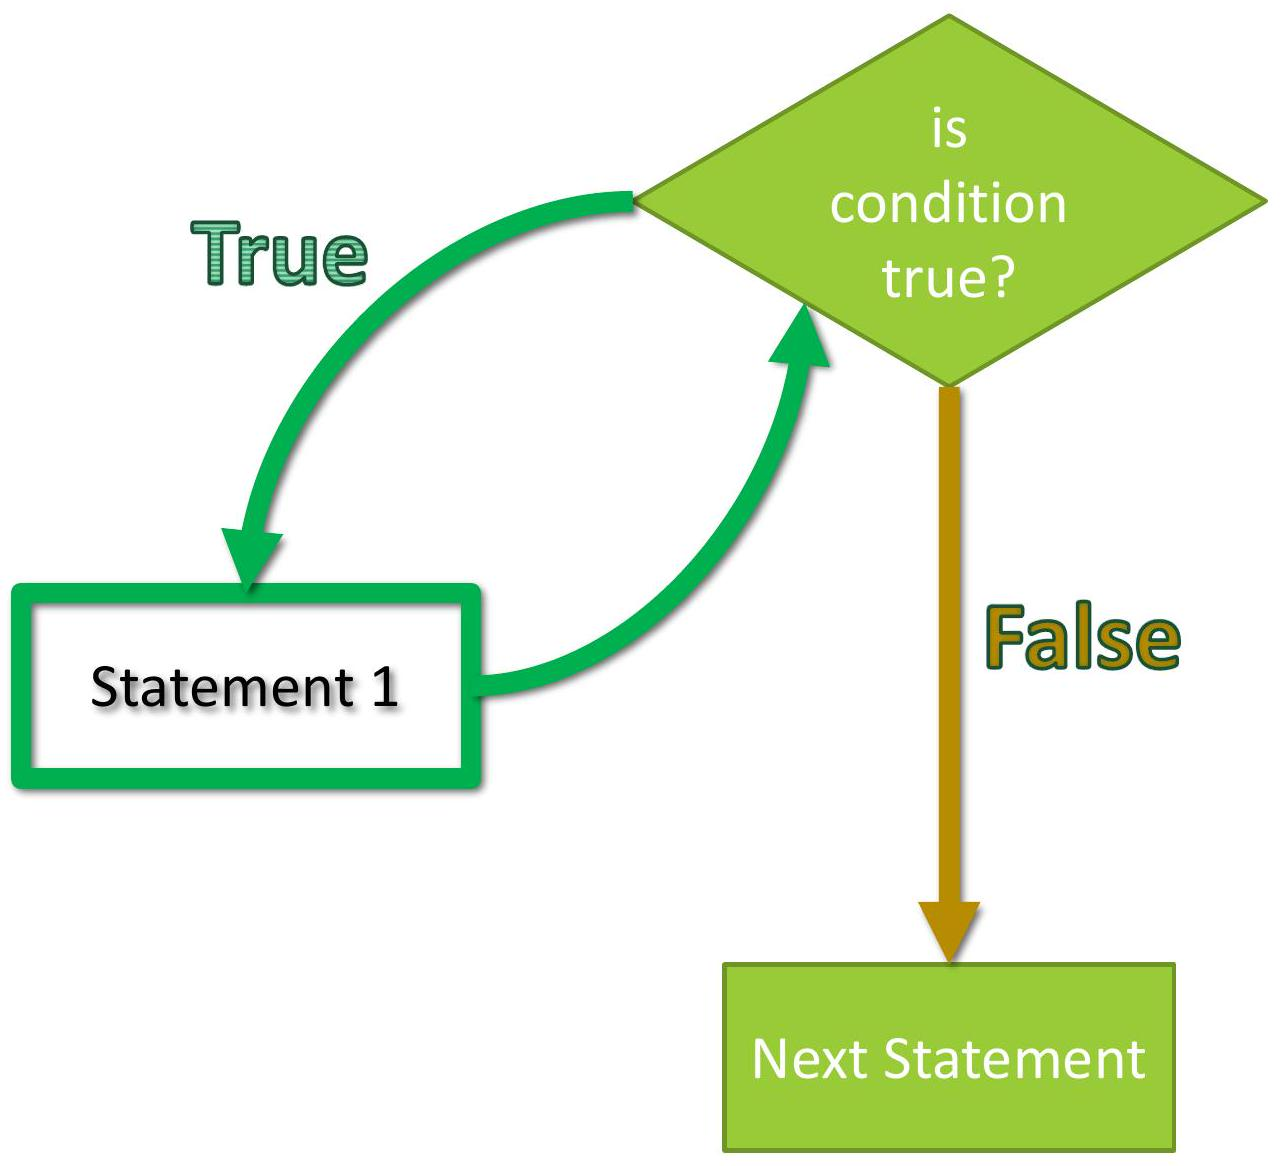
\includegraphics[width=0.6\textwidth]{../images/While-Loop-Flowchart.jpg}

This control flow applies equally to while and for loops.
\end{frame}

\begin{frame}[fragile]
\frametitle{For Loop Syntax}
\textbf{Example: Count to 10}
\begin{minted}[fontsize=\small]{cpp}
#include <iostream>
using namespace std;

int main() {
    for(int i = 1; i <= 10; i++)
        cout << i << endl;
    
    return 0;
}
\end{minted}
\pause

\textbf{Output:} 1, 2, 3, 4, 5, 6, 7, 8, 9, 10 (each on separate line)
\end{frame}

\begin{frame}[fragile]
\frametitle{For Loop Components Breakdown}
\begin{minted}[fontsize=\small]{cpp}
for(int i = 1; i <= 10; i++)
\end{minted}
\pause

\textbf{Three components (separated by semicolons):}
\begin{enumerate}
\item \texttt{int i = 1;} - \textbf{Initialization:} Sets counter starting value\pause
\item \texttt{i $\leq$ 10;} - \textbf{Condition:} Loop continues while true\pause
\item \texttt{i++} - \textbf{Update:} Runs at end of each iteration
\end{enumerate}
\end{frame}

\section{Scope and Best Practices}

\begin{frame}
\frametitle{Variable Scope: Context}
Variables declared in the for loop header have limited lifetime.\pause

They only exist within the loop structure itself.\pause

Next slide illustrates what happens when you try to access a loop variable outside its scope.
\end{frame}

\begin{frame}[fragile]
\frametitle{Variable Scope: The Loop Variable}
\begin{minted}[fontsize=\small]{cpp}
for(int i = 1; i <= 10; i++)
    cout << i << endl;

cout << i << endl;  // ERROR!
\end{minted}
\pause

\textbf{Compiler error:}
\begin{verbatim}
error: 'i' was not declared in this scope
\end{verbatim}
\pause

The variable \texttt{i} only exists inside the for loop. It is destroyed after the loop ends.
\end{frame}

\begin{frame}
\frametitle{Scope Visualization Context}
Understanding scope helps prevent common programming errors.\pause

Think of scope as a boundary: variables created inside cannot escape outside.\pause

Next slide shows a visual representation of this concept.
\end{frame}

\begin{frame}
\frametitle{Scope Visualization}
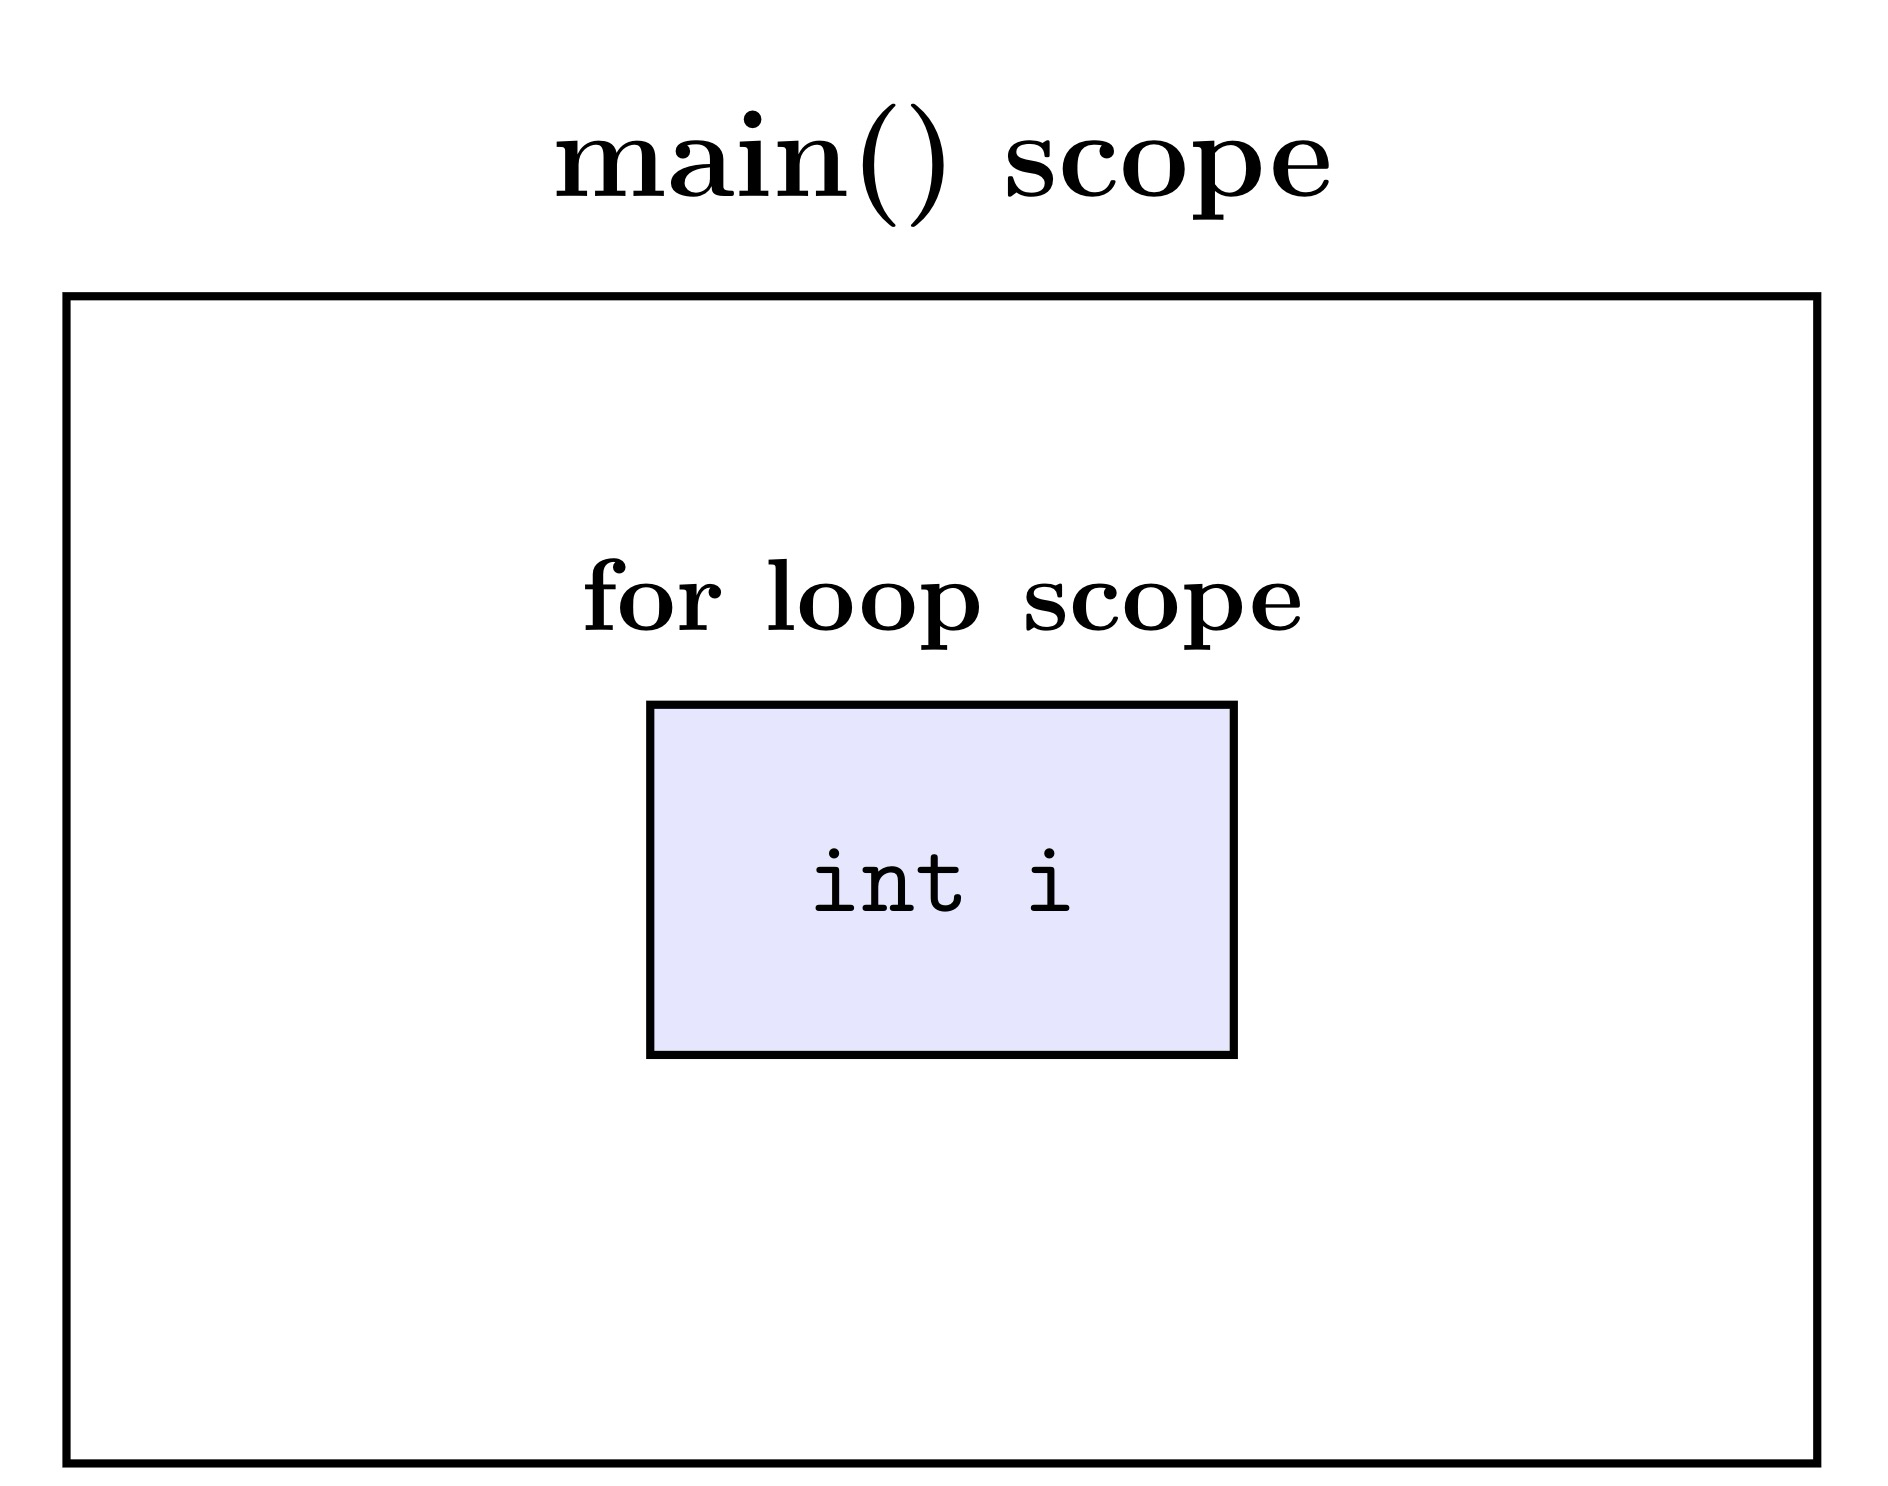
\includegraphics[width=\textwidth]{../images/scope-loop.png}

Variable \texttt{i} is born inside the for loop and dies when the loop ends.
\end{frame}

\begin{frame}[fragile]
\frametitle{Converting While to For: Leap Years}
\textbf{While loop version:}
\begin{minted}[fontsize=\scriptsize]{cpp}
int y1 = 1893;
int y2 = 1915;
while(y1 <= y2) {
    if(y1 % 400 == 0 || (y1 % 4 == 0 && y1 % 100 != 0))
        cout << y1 << endl;
    y1++;
}
\end{minted}
\pause

\textbf{For loop version:}
\begin{minted}[fontsize=\scriptsize]{cpp}
int y1 = 1893;
int y2 = 1915;
for(int i = y1; i <= y2; i++) {
    if(i % 400 == 0 || (i % 4 == 0 && i % 100 != 0))
        cout << i << endl;
}
\end{minted}
\end{frame}

\begin{frame}[fragile]
\frametitle{Converting While to For: Arithmetic Sequence}
\textbf{For loop version:}
\begin{minted}[fontsize=\scriptsize]{cpp}
int t = 12;
int d = -2;
int n = 10;
int sum = t;

cout << "Term\t\tSum\n";

for(int i = 1; i <= n; i++) {
    cout << t << "\t\t" << sum << endl; 
    t = t + d;
    sum = sum + t;
}
\end{minted}

More concise than while loop when you know the exact iteration count.
\end{frame}

\begin{frame}
\frametitle{Compound Assignment Operators}
C++ provides shortcuts for common operations.\pause

\begin{center}
\begin{tabular}{|l|l|l|}
\hline
\textbf{Operator} & \textbf{Example} & \textbf{Equivalent to} \\
\hline
+= & \texttt{x += 6;} & \texttt{x = x + 6;} \\
\hline
-= & \texttt{x -= 10;} & \texttt{x = x - 10;} \\
\hline
*= & \texttt{x *= 2;} & \texttt{x = x * 2;} \\
\hline
/= & \texttt{x /= 2;} & \texttt{x = x / 2;} \\
\hline
\end{tabular}
\end{center}
\pause

These perform the operation AND store the result in one step.
\end{frame}

\begin{frame}[fragile]
\frametitle{Compound Operators: Examples}
\begin{minted}[fontsize=\small]{cpp}
int x = 10;

x += 6;   // x is now 16
x -= 10;  // x is now 6
x *= 2;   // x is now 12
x /= 2;   // x is now 6
\end{minted}
\pause

\textbf{Common usage in loops:}
\begin{minted}[fontsize=\small]{cpp}
sum += value;  // Add to running total
count++;       // Increment counter
\end{minted}
\end{frame}

\begin{frame}[fragile]
\frametitle{Common Syntax Error: Commas}
\textbf{WRONG (commas):}
\begin{minted}[fontsize=\small]{cpp}
for(int i = 0, i < 10, i++) {
    cout << i << '\n';
}
\end{minted}
\pause

\textbf{Compiler error: Will not compile!}\pause

\textbf{CORRECT (semicolons):}
\begin{minted}[fontsize=\small]{cpp}
for(int i = 0; i < 10; i++) {
    cout << i << '\n';
}
\end{minted}

Remember: semicolons separate the three for loop components.
\end{frame}

\section{Nested Loops}

\begin{frame}
\frametitle{Nested Loops: Context}
Loops can be placed inside other loops, creating nested structures.\pause

Each iteration of the outer loop runs the entire inner loop.\pause

This is useful for working with multi-dimensional data like grids, tables, or coordinate systems.\pause

Next slides show examples with different nesting depths.
\end{frame}

\begin{frame}[fragile]
\frametitle{Nested Loops: Double Loop Example}
\textbf{Predict the output:}
\begin{minted}[fontsize=\small]{cpp}
int base = 8;
for(int i = 0; i < base; i++) {
    for(int j = 0; j < base; j++) {
        cout << i << "," << j << endl;
    }
}
\end{minted}
\pause

\textbf{Explanation:}
\begin{itemize}
\item Outer loop (i) runs 8 times
\item For each i, inner loop (j) runs 8 times
\item Total: $8 \times 8 = 64$ lines of output
\item Pattern: (0,0), (0,1), ..., (0,7), (1,0), (1,1), ..., (7,7)
\end{itemize}
\end{frame}

\begin{frame}[fragile]
\frametitle{Nested Loops: Triple Loop Example}
\textbf{Predict the output:}
\begin{minted}[fontsize=\scriptsize]{cpp}
int testValue = 0;
for(int i = 0; i < 8; i++) {
    for(int j = 0; j < 9; j++) {
        for(int k = 0; k < 10; k++) {
            testValue++;
        }
    }
}
cout << testValue << endl;
\end{minted}
\pause

\textbf{Answer:} 720\pause

\textbf{Calculation:} $8 \times 9 \times 10 = 720$ iterations
\end{frame}

\begin{frame}
\frametitle{Nested Loop Visualization Context}
Nested loops create a grid-like iteration pattern.\pause

The outer loop controls rows, inner loop controls columns.\pause

Next slide visualizes this concept.
\end{frame}

\begin{frame}
\frametitle{Nested Loop Visualization}
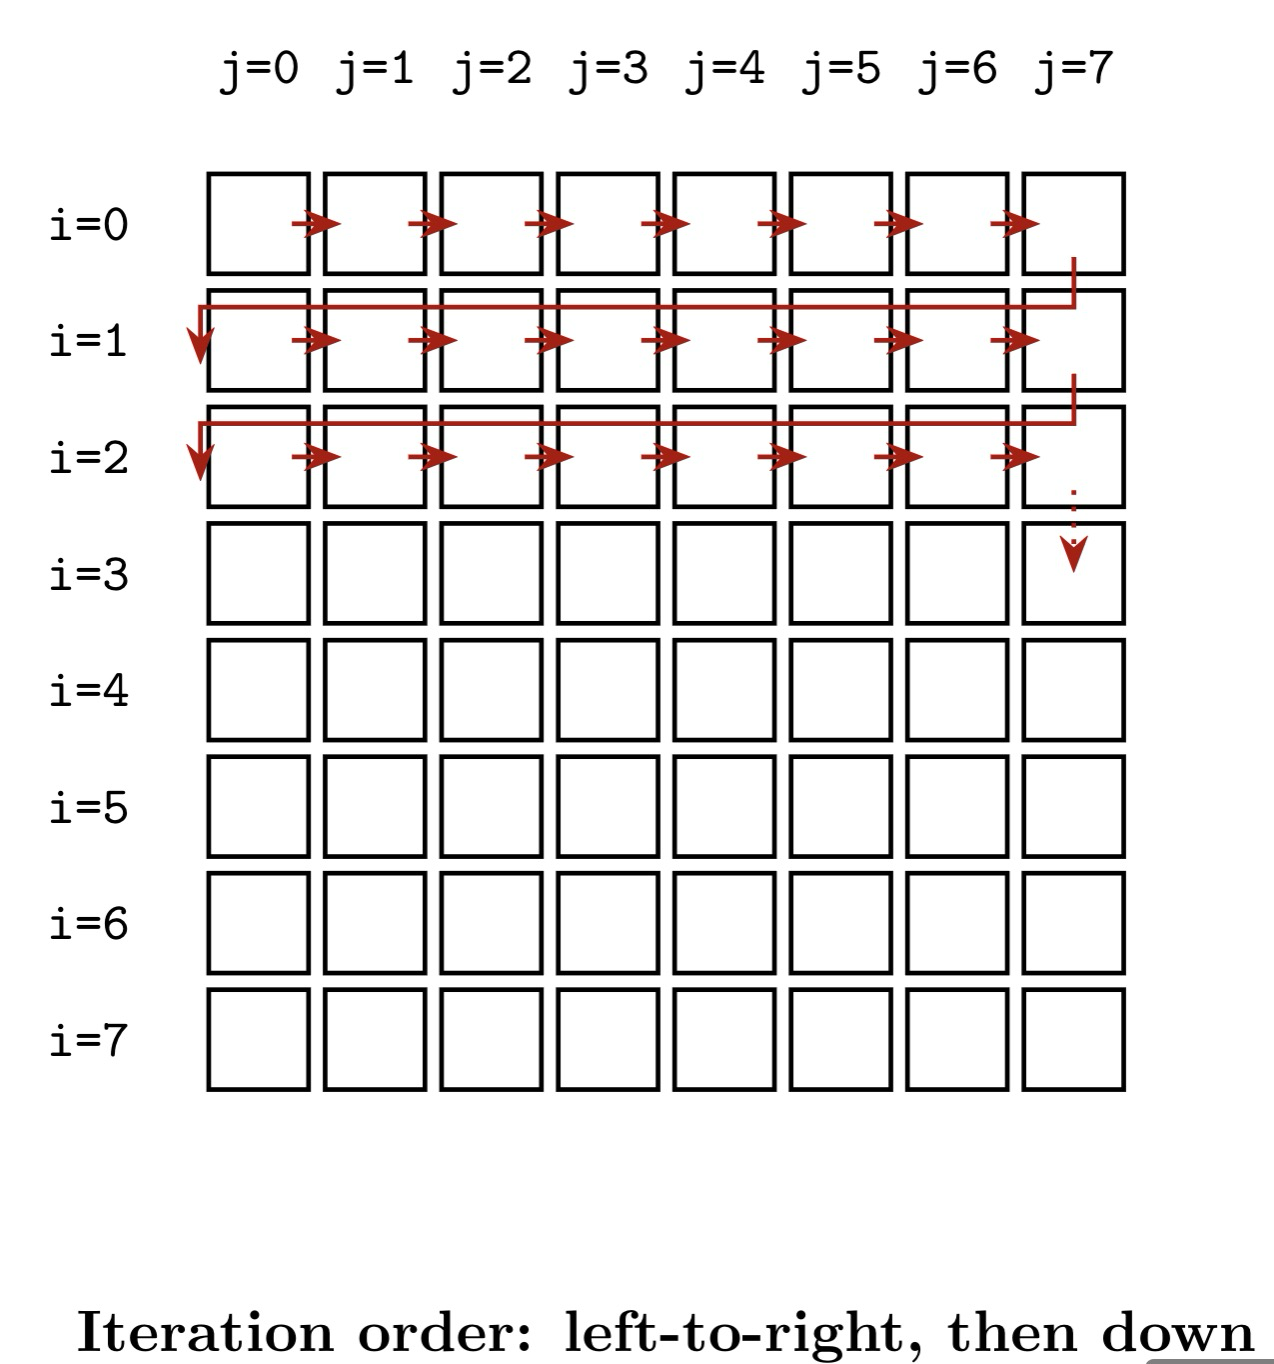
\includegraphics[width=\textwidth]{../images/Nested-Loop.png}

Each row represents one iteration of the outer loop.
\end{frame}

\section{Practice Exercises}

\begin{frame}[fragile]
\frametitle{Exercise 1: Factors}
\textbf{Exercise File:} \texttt{01\_factors.cpp} (Template with TODOs)

\textbf{Objective:} Output all factors of a positive integer without trailing comma.\pause

\begin{minted}[fontsize=\scriptsize, frame=lines, linenos, breaklines]{cpp}
#include <iostream>
using namespace std;

int main() {
    int n = 24;
    
    // TODO 1: Create a for loop from 1 to n
    // TODO 2: Check if i divides n evenly (use modulo)
    // TODO 3: Print i followed by comma (except for last)
    // Hint: Check if i equals n to avoid trailing comma
    
    return 0;
}
\end{minted}

\textbf{Expected output for n=24:} 1, 2, 3, 4, 6, 8, 12, 24
\end{frame}

\begin{frame}[fragile]
\frametitle{Exercise 2: Output a Square}
\textbf{Exercise File:} \texttt{02\_square.cpp} (Template with TODOs)

\textbf{Objective:} Use nested loops to create a square of X characters.\pause

\begin{minted}[fontsize=\scriptsize, frame=lines, linenos, breaklines]{cpp}
#include <iostream>
using namespace std;

int main() {
    int length = 4;
    
    // TODO 1: Create outer loop for rows (i from 0 to length)
    // TODO 2: Create inner loop for columns (j from 0 to length)
    // TODO 3: Print 'X' in inner loop
    // TODO 4: Print newline after inner loop completes
    
    return 0;
}
\end{minted}

\textbf{Expected output for length=4:}
\begin{verbatim}
XXXX
XXXX
XXXX
XXXX
\end{verbatim}
\end{frame}

\begin{frame}[fragile]
\frametitle{Exercise 3: Output a Triangle}
\textbf{Exercise File:} \texttt{03\_triangle.cpp} (Template with TODOs)

\textbf{Objective:} Create isosceles right triangle using nested loops.\pause

\begin{minted}[fontsize=\scriptsize, frame=lines, linenos, breaklines]{cpp}
#include <iostream>
using namespace std;

int main() {
    int leg = 4;
    
    // TODO 1: Outer loop for rows (i from leg down to 1)
    // TODO 2: Inner loop for columns (j from 0 to i)
    // TODO 3: Print 'X' in inner loop
    // TODO 4: Print newline after inner loop
    
    return 0;
}
\end{minted}

\textbf{Expected output for leg=4:}
\begin{verbatim}
XXXX
XXX
XX
X
\end{verbatim}
\end{frame}

\begin{frame}[fragile]
\frametitle{Exercise 4: Temperature Conversion}
\textbf{Exercise File:} \texttt{04\_temperature.cpp} (Template with TODOs)

\textbf{Objective:} Display table of 20 Fahrenheit to Celsius conversions.\pause

\begin{minted}[fontsize=\scriptsize, frame=lines, linenos, breaklines]{cpp}
#include <iostream>
using namespace std;

int main() {
    float fahrenheit = 20.0;
    float celsius;
    
    cout << "Fahrenheit\tCelsius\n";
    
    // TODO 1: Create for loop (i from 0 to 19)
    // TODO 2: Calculate celsius = (5.0/9.0)*(fahrenheit-32.0)
    // TODO 3: Print fahrenheit and celsius
    // TODO 4: Increment fahrenheit by 4
    
    return 0;
}
\end{minted}

Start at 20°F, increment by 4°. Use float for decimal precision.
\end{frame}

\begin{frame}[fragile]
\frametitle{Exercise 5: Sum of Multiples (Project Euler \#1)}
\textbf{Exercise File:} \texttt{05\_multiples.cpp} (Template with TODOs)

\textbf{Problem:} Find sum of all multiples of 3 or 5 below 1000.\pause

\begin{minted}[fontsize=\scriptsize, frame=lines, linenos, breaklines]{cpp}
#include <iostream>
using namespace std;

int main() {
    int sum = 0;
    
    // TODO 1: Create for loop (i from 1 to 999)
    // TODO 2: Check if i is divisible by 3 OR 5
    // TODO 3: If true, add i to sum
    // TODO 4: Print final sum
    
    return 0;
}
\end{minted}

\textbf{Hint:} Number 15 is divisible by both 3 and 5, count it once.
\end{frame}

\begin{frame}[fragile]
\frametitle{Exercise 6: Even Fibonacci Sum (Project Euler \#2)}
\textbf{Exercise File:} \texttt{06\_fibonacci.cpp} (Template with TODOs)

\textbf{Problem:} Sum of even Fibonacci terms below 1,000,000.\pause

\begin{minted}[fontsize=\scriptsize, frame=lines, linenos, breaklines]{cpp}
#include <iostream>
using namespace std;

int main() {
    int a = 1, b = 2;
    int sum = 0;
    
    // TODO 1: While loop: continue while b < 1000000
    // TODO 2: If b is even, add to sum
    // TODO 3: Calculate next Fibonacci: temp = a + b
    // TODO 4: Update a = b, b = temp
    // TODO 5: Print final sum
    
    return 0;
}
\end{minted}

\textbf{Sequence:} 1, 2, 3, 5, 8, 13, 21, 34, 55, 89, ...
\end{frame}

\begin{frame}[fragile]
\frametitle{Exercise 7: Prime Factors (Project Euler \#3)}
\textbf{Exercise File:} \texttt{07\_primeFactors.cpp} (Template with TODOs)

\textbf{Problem:} Find largest prime factor of 600851475143.\pause

\begin{minted}[fontsize=\scriptsize, frame=lines, linenos, breaklines]{cpp}
#include <iostream>
using namespace std;

int main() {
    unsigned long long testNum = 600851475143;
    unsigned long long current_n = 2;
    unsigned long long largestPrime = 0;
    
    // TODO 1: While loop: continue while testNum > 1
    // TODO 2: If testNum divisible by current_n
    // TODO 3:   Update largestPrime = current_n
    // TODO 4:   Divide testNum by current_n
    // TODO 5: Else increment current_n
    // TODO 6: Print largestPrime
    
    return 0;
}
\end{minted}
\end{frame}

\begin{frame}
\frametitle{Prime Factors Algorithm Context}
Finding prime factors uses division to break down numbers.\pause

Algorithm repeatedly divides by smallest possible divisor.\pause

Because we test divisors in order (2, 3, 4, ...), any divisor that works must be prime. Why?\pause

If it had smaller factors, we would have already divided them out.\pause

Next slide shows conceptual breakdown with smaller number.
\end{frame}

\begin{frame}[fragile]
\frametitle{Prime Factors: How It Works}
\textbf{Example with 12:}
\begin{verbatim}
testNum = 12, current_n starts at 2

12 ÷ 2 = 6 (remainder 0) → Found prime factor 2
testNum becomes 6

6 ÷ 2 = 3 (remainder 0) → Found prime factor 2
testNum becomes 3

3 ÷ 2 = 1 remainder 1 → Not divisible, try next
current_n becomes 3

3 ÷ 3 = 1 (remainder 0) → Found prime factor 3
testNum becomes 1, DONE
\end{verbatim}

Prime factors of 12: 2, 2, 3 (multiply: $2 \times 2 \times 3 = 12$)
\end{frame}

\begin{frame}
\frametitle{Summary}
\textbf{Key takeaways:}
\begin{itemize}
\item For loops package initialization, condition, update in one line
\item Best for known iteration counts
\item Loop variables have limited scope (exist only in loop)
\item Compound operators (+=, -=, *=, /=) save typing
\item Use semicolons, not commas, in for loop header
\item Nested loops multiply iteration counts
\item Convert while to for when iteration count is known
\end{itemize}
\pause

\textbf{Practice makes perfect:} Complete all seven exercises to master for loops!
\end{frame}

\end{document}
